Tras exponer la implementación de los diferentes módulos del sistema, este capítulo detalla su evaluación y la comparación entre las diferentes versiones propuestas.

En esta línea, inicialmente se explica el sistema de evaluación implementado, tras lo que se exponen los resultados de evaluación y las conclusiones derivadas de dichos resultados. 

\section{Sistema de evaluación}
Evaluar el sistema presenta un desafío inherente a su naturaleza, ya que se debe evaluar la capacidad de este para responder preguntas en lenguaje natural. Para resolver esta problemática, se han definido una serie de métricas utilizando para ello la metodología de evaluación ofrecida por la librería LangSmith sobre un dataset anotado manualmente que actúa como respuesta correcta o \textit{ground truth}.

\subsection{Métricas de evaluación}
Siguiendo los principios etablecidos en la Sección \colorbox{yellow}{(sección antecedentes evaluación)}, se han definido las siguientes métricas para cada agente:

\paragraph{LLM juez}Consiste en utilizar un agente evaluador cuya función sea valorar el resultado obtenido por el agente evaluado.

Esta métrica incorpora variabilidad de precisión adicional, ya que el agente evaluador también contiene una tasa de error. Para minimizar dicha tasa, se han anotado las respuestas esperadas como listas textuales con los conceptos necesarios a incluir en la respuesta del agente. De esta forma, el agente juez genera una respuesta estructurada que contiene un argumento booleano para cada concepto requerido, indicando si se incluye en la respuesta generada, calculando así una precisión medible para la calidad de la respuesta.

Cabe destacar que el juez marcará como incorrecto todo concepto más abstracto que el anotado, aún si conceptualmente el significado es equivalente. Por ejemplo, si se anota que la función del proyecto es proporcionar herramientas de modelos de lenguaje generativos para el equipo de desarrolladores, una respuesta sobre proporcionar herramientas de inteligencia artificial para el equipo sería considerada incorrecta.

\paragraph{Precisión de herramientas}Se comparan las herramientas utilizadas por un agente para responder una pregunta con el listado de herramientas anotado como perfecto, calculando dos métricas posibles: 
\begin{itemize}
  \item Precisión de herramientas necesarias: indica la cantidad de herramientas necesarias utilizadas, favoreciendo el uso de estas.
  \item Precisión de herramientas innecesarias: indica la cantidad de herrmientas innecesarias ignoradas, desfavoreciendo el uso de estas.  
\end{itemize}

Por ejemplo, un agente podría tener 5 herramientas disponibles, de las cuales 2 son necesarias, 2 son innecesarias, y otra no se clasifica en ninguno de los dos grupos, puediendo ser de utilidad pero no indispensable. Si este llama a 1 necesaria y 2 innecesarias, la precisión necesaria sería de 0.5, mientras que la innecesaria sería de 0.0. La media total sería de 0.25. El uso de la herramienta no clasificada no varía ninguna precisión.  

\paragraph{Precisión de alucinación}Los modelos tienden a responder las consultas realizadas aún si no contienen el conocimiento necesario para ello. Para evaluar esto, se han anotado algunas preguntas que son imposibles de responder con la información a la que el agente tiene acceso. Ante la consulta: \texttt{¿Qué flujo de despliegue contínuo se utiliza?}, el agente no podrá responder correctamente porque no existe dicho flujo.

Para evaluar esto, un agente juez determina si la respuesta del agente realmente intenta responder a la pregunta o por el contrario indica que no se dispone de la suficiente información.

\paragraph{Precisión de citado}Constituye la cantidad de documentos citados en la respuesta que estaban anotados como necesarios.   

\subsection{Implementación de evaluación}
Se ha incorporado el sistema de evaluación de LangSmith en la arquitectura agéntica utilizada. Para ello, se ha creado un dataset en dicha plataforma para cada agente con los datos ground truth anotados. La Figura \ref{} muestra un esquema de dicho mecanismo

\begin{figure}[h]
\centering
\adjustbox{center=\textwidth}{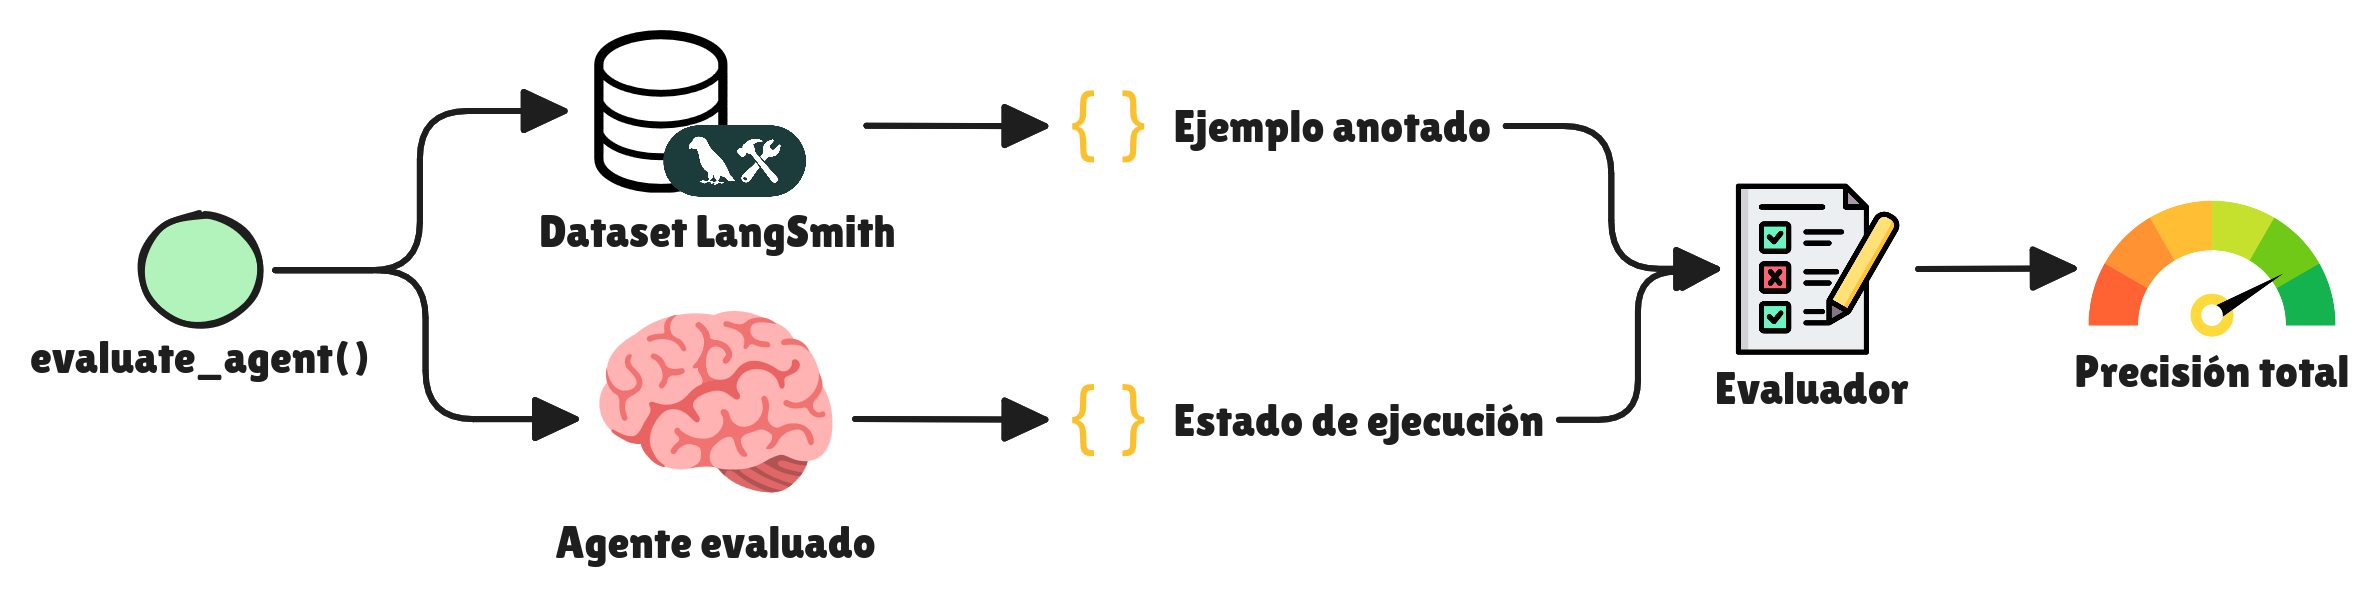
\includegraphics[width=1\linewidth]{figures/evaluacion.png}}
\caption{Mecanismo de evaluación de agentes}
\label{fig:mem_1}
\end{figure}

Se utiliza la función \opus{evaluate\_agent()} heredada por todos los agentes, la cual define una serie de instancias \opus{BaseEvaluator} que se ejecutarán sobre el dataset del agente. El Listado \ref{lst:evaluate} ilustra la evaluación de los agentes especializados, donde se declaran los evaluadores a utilizar.

\begin{lstlisting}[caption={Evaluación de agentes especializados},label={lst:evaluate}]
async def evaluate_agent(self, langsmith_client: Client):
    evaluators = [
        ToolPrecisionEvaluator(self.get_tools_from_run_state),
        JudgeLLMEvaluator(),
        CiteEvaluator()
    ]
    result = await self.call_agent_evaluation(langsmith_client, evaluators)
    return result
\end{lstlisting}

Esta función invoca \opus{call\_agent\_evaluation()}, heredado por todos los agentes (Listado \ref{lst:call_evaluation}), que ejecuta la función de evaluación de LangSmith para aplicar las funciones de evaluación sobre cada estado final de ejecución y ejemplo anotado.

\begin{lstlisting}[caption={Llamada a evaluación de agentes},label={lst:call_evaluation}]
async def call_agent_evaluation(self, langsmith_client: Client, 
                               evaluators: List[BaseEvaluator], ...):
    ...
    run_function = self.execute_from_dataset
    results = await aevaluate(
        run_function,
        data=data,
        client=langsmith_client,
        evaluators=evaluator_functions,
        max_concurrency=max_conc,
        experiment_prefix=evaluation_name,
    )
    return results
\end{lstlisting}

El Listado \ref{lst:cite_evaluator} muestra la implementación del evaluador de citas, donde se utilizan el estado de ejecución y el ejemplo anotado para calcular la precisión.

\begin{lstlisting}[caption={Evaluador de citas},label={lst:cite_evaluator}]
class CiteEvaluator(BaseEvaluator):
    async def evaluate(self, run: Run, example: Example) -> EvaluationResults:
        run_state = run.outputs.get("run_state")
        expected_cites = example.outputs.get("cite")
        ...
        return EvaluationResults(
            results=[
                EvaluationResult(
                    key="cite_precision",
                    score=StrictFloat(citation_score)
                )
            ]
        )
\end{lstlisting}




\subsection{Dataset anotado}
La captura de dicho dataset se ha realizado en una hoja de cálculo de Google Drive. Esta hoja se ha descargado posteriormente en formato de valores separados por coma (CSV), y se ha subido como dataset de LangSmith. 

La captura constituye de 46 ejemplos para el agente principal (el sistema completo), y aproximadamente 10 ejemplos para los agentes individuales. Para ello se han utilizado las preguntas anotadas en la captura de requisitos, filtrando y modificando en algunos casos las preguntas para ser lo suficientemente específicas como para tener una respuesta exacta, pero a su vez con cierto grado de complejidad que requiera un razonamiento sobre la consulta. Se han utilizado las siguientes consideraciones sobre cada agente: 

\begin{itemize}
  \item\textbf{Agente principal: }Se han identificado tres tipos de preguntas: aquellas que se pueden responder consultando una única fuente de datos, las que requieren múltiples fuentes de datos, y las que requieren múltiples fuentes de datos en un orden sequencial, dependiendo la entrada de uno de la salida del otro.   
  \item\textbf{Planificador: }Para este agente se ha anotado la respuesta como el plan generado para un ejemplo de ejecución, incluyendo la pregunta y el estado de ejecución, siendo este último la información de la que se dispone y el plan actual.

De esta forma, se han identificado tres escenarios: preguntas donde se requiere un solo paso, preguntas donde se requieren varios pasos, y preguntas a medio completar donde se requiere que el agente genere el siguiente paso o decida finalizar el plan. 
\item\textbf{Orquestador: }Este agente se ha evaluado utilizando los agentes seleccionados para ejecutar como herramientas. Para ello se han incluido preguntas de todas las temáticas, evaluando qué agentes llamar en cada caso:

\begin{itemize}
    \item \textbf{Tareas de agente único: }Se ha definido una consulta relacionada únicamente con cada agente especializado. 
    \item \textbf{Tareas multi-agente:}
    \begin{itemize}
        \item Información general: \opus{file_system_agent} principalmente
        \item Entorno y despliegue: \opus{file_system_agent} + \opus{code_agent}
        \item Gestión del proyecto: \opus{file_system_agent} + otros agentes según el caso
        \item Estándares y prácticas: \opus{file_system_agent} + \opus{confluence_agent} si es frontend
        \item Documentación: \opus{file_system_agent}
        \item Arquitectura del sistema: \opus{code_agent} + \opus{file_system_agent} en la mayoría
        \item Tareas de frontend: \opus{confluence_agent} + \opus{google_drive_agent}
    \end{itemize}
  \end{itemize}
\item\textbf{Agente sistema de ficheros, Confluence y Google Drive}: En los casos sencillos es necesario únicamente la herramienta de leer páginas. En los más desafiantes se requiere de las herramientas de búsqueda.
\item\textbf{Agente GitLab: }Se han incluido ejemplos donde este debe llamar primero a la herramienta de obtener información sobre los usuarios en caso de necesitarlo para especificar el nombre de usuario en otras herramientas.
\item\textbf{Agente código: }En los casos sencillos los chunks relevantes deberían estar incluidos en el prompt de entrada, mientras que en los más complejos debería buscar información adicional. 
\end{itemize}
\section{Resultados obtenidos}
En esta sección se presentan los resultados obtenidos mediante el sistema implementado. En primera instancia se exponen los resultados de evaluación correspondientes a la versión inicial de cada agente, contrastados con una segunda versión que incorpora un prompt optimizado. Posteriormente se evalúan los distintos sistemas de orquestación desarrollados. Finalmente se analizan las mejoras introducidas en el sistema.
\subsection{Mejora de primera versión}
Una vez desarrollado un sistema mínimo compuesto por los agentes especializados, un planificador y un orquestador, se evaluó su rendimiento con las métricas establecidas. Primero se procedió a mejorar los agentes especializados, tras lo que se incorporó el prompting few-shot en el orquestador y planificador.

\subsubsection{Agentes especializados}
La Figura \ref{} ilustra la precisión para las métricas juez, citación, alucinación y gasto promedio en millares de tokens para los agentes especializados. Todas las evaluaciones fueron ejecutadas dos veces para reducir variaciones. 

\begin{figure}[hbtp]
\centering

% Definir estilos comunes para todos los gráficos
\pgfplotsset{
    mybar/.style={
        ylabel=,  
        xlabel=,
        x tick label style={font=\tiny},
        yticklabel style={font=\tiny},
        ymin=0,
        enlarge x limits=0.12,
        ybar=4pt,
        bar width=5pt,
        symbolic x coords={Code, Confluence, FileSystem, GDrive, Gitlab},
        xtick={Code, Confluence, FileSystem, GDrive, Gitlab},
        x tick label style={rotate=45, anchor=east, font=\scriptsize},
        width=4.3cm,
        height=4.5cm,
        grid=major,
        grid style={dashed, gray!30},
        tick label style={font=\scriptsize},
        legend style={draw=none},
        scale only axis,
    }
}

% Primera fila con tres gráficos usando minipage
\begin{minipage}{0.32\textwidth}
\centering
\subfloat[LLM Juez\label{fig:llm_juez}]{
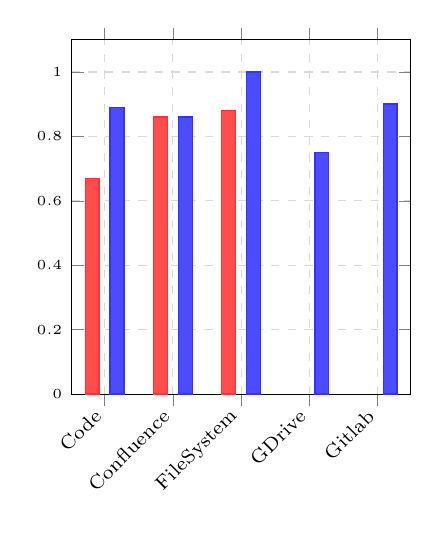
\begin{tikzpicture}
\begin{axis}[
    mybar,
    ymax=1.1,
    ytick={0,0.2,0.4,0.6,0.8,1.0},
]
\addplot[
    fill=red!70,
    draw=red!80,
    line width=0.5pt
] coordinates {
    (Code, 0.67)
    (Confluence, 0.86)
    (FileSystem, 0.88)
    (GDrive, nan)
    (Gitlab, nan)
};
\addplot[
    fill=blue!70,
    draw=blue!80,
    line width=0.5pt
] coordinates {
    (Code, 0.89)
    (Confluence, 0.86)
    (FileSystem, 1.0)
    (GDrive, 0.75)
    (Gitlab, 0.9)
};
\end{axis}
\end{tikzpicture}
}
\end{minipage}
\begin{minipage}{0.32\textwidth}
\centering
\subfloat[Precisión Citas\label{fig:precision_citas}]{
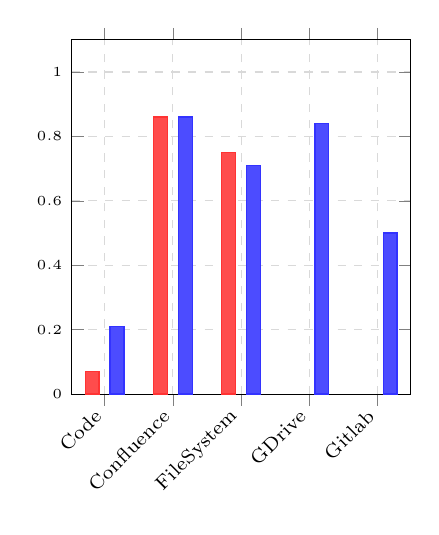
\begin{tikzpicture}
\begin{axis}[
    mybar,
    ymax=1.1,
    ytick={0,0.2,0.4,0.6,0.8,1.0},
]
\addplot[
    fill=red!70,
    draw=red!80,
    line width=0.5pt
] coordinates {
    (Code, 0.07)
    (Confluence, 0.86)
    (FileSystem, 0.75)
    (GDrive, nan)
    (Gitlab, nan)
};
\addplot[
    fill=blue!70,
    draw=blue!80,
    line width=0.5pt
] coordinates {
    (Code, 0.21)
    (Confluence, 0.86)
    (FileSystem, 0.71)
    (GDrive, 0.84)
    (Gitlab, 0.5)
};
\end{axis}
\end{tikzpicture}
}
\end{minipage}
\begin{minipage}{0.32\textwidth}
\centering
\subfloat[Precisión Herramientas\label{fig:precision_herramientas}]{
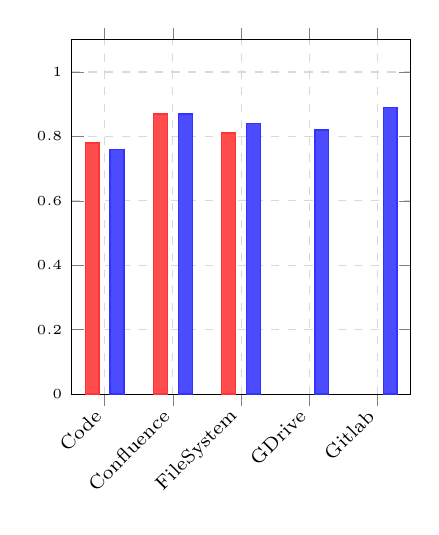
\begin{tikzpicture}
\begin{axis}[
    mybar,
    ymax=1.1,
    ytick={0,0.2,0.4,0.6,0.8,1.0},
]
\addplot[
    fill=red!70,
    draw=red!80,
    line width=0.5pt
] coordinates {
    (Code, 0.78)
    (Confluence, 0.87)
    (FileSystem, 0.81)
    (GDrive, nan)
    (Gitlab, nan)
};
\addplot[
    fill=blue!70,
    draw=blue!80,
    line width=0.5pt
] coordinates {
    (Code, 0.76)
    (Confluence, 0.87)
    (FileSystem, 0.84)
    (GDrive, 0.82)
    (Gitlab, 0.89)
};
\end{axis}
\end{tikzpicture}
}
\end{minipage}

\vspace{0.2cm}

% Segunda fila con dos gráficos centrados
\begin{minipage}{0.32\textwidth}
\centering
\subfloat[Alucinación\label{fig:halucinacion}]{
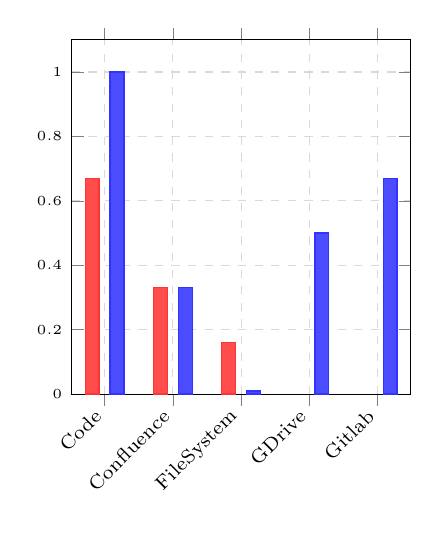
\begin{tikzpicture}
\begin{axis}[
    mybar,
    ymax=1.1,
    ytick={0,0.2,0.4,0.6,0.8,1.0},
]
\addplot[
    fill=red!70,
    draw=red!80,
    line width=0.5pt
] coordinates {
    (Code, 0.67)
    (Confluence, 0.33)
    (FileSystem, 0.16)
    (GDrive, nan)
    (Gitlab, nan)
};
\addplot[
    fill=blue!70,
    draw=blue!80,
    line width=0.5pt
] coordinates {
    (Code, 1.0)
    (Confluence, 0.33)
    (FileSystem, 0.01)
    (GDrive, 0.5)
    (Gitlab, 0.67)
};
\end{axis}
\end{tikzpicture}
}
\end{minipage}
\hspace{0.05\textwidth}
\begin{minipage}{0.32\textwidth}
\centering
\subfloat[Tokens Utilizados (millares)\label{fig:tokens}]{
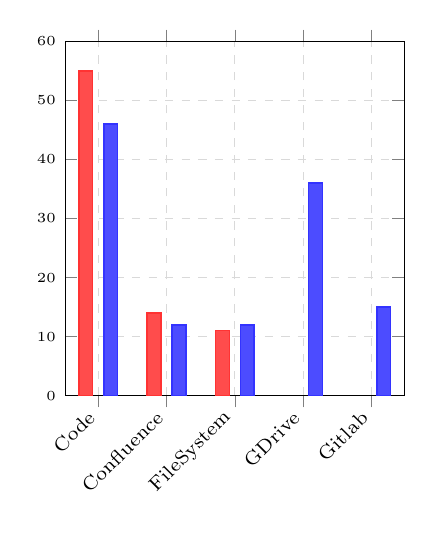
\begin{tikzpicture}
\begin{axis}[
    mybar,
    ymax=60,
    ytick={0,10,20,30,40,50,60},  % Para el gráfico de tokens
]
\addplot[
    fill=red!70,
    draw=red!80,
    line width=0.5pt
] coordinates {
    (Code, 55)
    (Confluence, 14)
    (FileSystem, 11)
    (GDrive, nan)
    (Gitlab, nan)
};
\addplot[
    fill=blue!70,
    draw=blue!80,
    line width=0.5pt
] coordinates {
    (Code, 46)
    (Confluence, 12)
    (FileSystem, 12)
    (GDrive, 36)
    (Gitlab, 15)
};
\end{axis}
\end{tikzpicture}
}
\end{minipage}

% Leyenda global centrada (simplificada)
\vspace{-0.2cm} % Justo antes del bloque de leyenda
\begin{center}

\begin{tikzpicture}
    \draw[fill=red!70,draw=red!80,line width=0.5pt] (0,0) rectangle (0.4,-0.25);
    \node[right] at (0.5,-0.125) {Inicial};
    \draw[fill=blue!70,draw=blue!80,line width=0.5pt] (2,0) rectangle (2.4,-0.25);
    \node[right] at (2.5,-0.125) {Mejorado};
\end{tikzpicture}
\end{center}

\caption{Comparación de métricas entre versión inicial y mejorada}
\label{fig:comparacion_metricas}
\end{figure}
\vspace{-0.2cm} 

Se observó que el gasto del agente de código era muy superior a los demás. Esto se debe a que se realizan varias consultas RAG para la misma pregunta. Se ajustó el prompt y la cantidad de chunks extraídos, ya que se observó que la mayoría del gasto venía de ejecuciones individuales prolongadas.

Por otro lado, la mejora del agnete Confluence representa el agente enfocado en el prompt caching. Aunque la precisión en todas las métricas es similar, el enfoque en prompt caching redució el uso y el gasto ligeramente. 

La mejora en el agente de sistema de ficheros representa la inclusión de la herramienta de RAG. 

\subsubsection{Prompting few-shot}
La Figura \ref{} ilustra la comparación para el agente planificador y orquestador tras incorporar el prompting few-shot. Como se puede observar, este mejoró considerablemente ambos agentes.

\subsection{Variaciones de orquestación}
Esta evaluación compara los diferentes enfoques de orquestación: planificación dividida, planificación unificada y el sistema sin planificación. Adicionalmente se incluye la evaluación del sistema con planificación dividida antes de implementar las mejoras de la sección anterior. 

Como se puede observar en la Figra \ref{}, las mejoras de la sección anterior mejoraron significativamente el sistema general. El prompting few-shot en los agentes superiores redució la cantidad de agentes utilizados, mejorando significativamente el costo total.

Los resultados de evaluación evidencian que el paso de planificación mejora le sistema. Más concretamente, la planificación unificada supera a la dividida. Esto significa que en este caso de uso, la divisió lógica del paso de planificació no es rentable, y es mejor que el agente planificador tenga directamente la máxima información posible para fundamentear su plan. 

\subsection{Integración de memoria}
Para la evaluación de este componente se ha dividido el dataset del agente principal en dos partes, en entrenamiento (80\%) y evaluación (20\%). El objetivo es analizar si las memorias de ejecuciones de las consultas del dataset de entrenamiento pueden mejorar el rendimiento en el dataset de evaluación. Por lo tanto, se ejecutó primero el sistema completo en el dataste de entrenamiento, acumulando memorias para este. Después, se ejecutó en el dataset de evaluación, para comparar el resultado con el sistema sin memoria.

Los resultados se ilustran en la Figura \ref{}. Como se puede observar, la inclusión de memorias del dataset de entrenamiento realmente mejoró la precisión respecto al sistema sin memoria.
































\clearpage

79, 78, 82,333
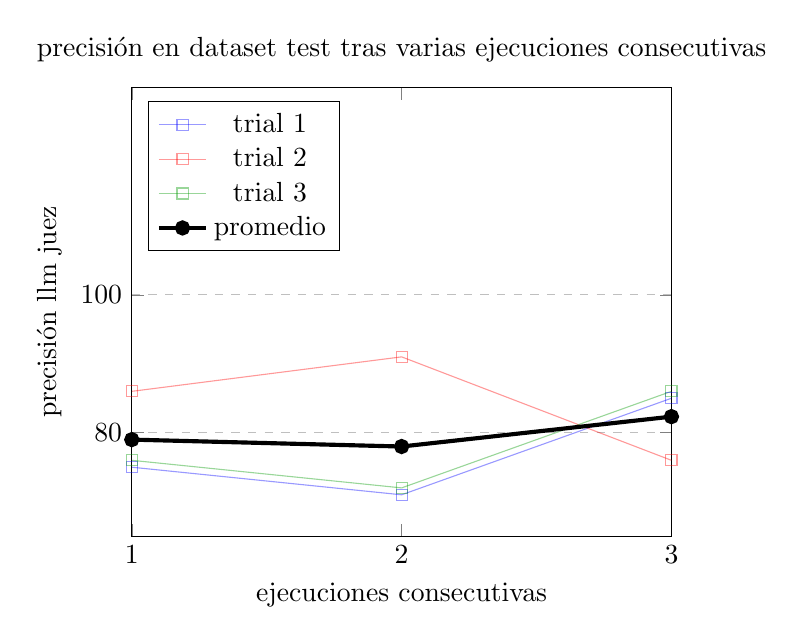
\begin{tikzpicture}
\begin{axis}[
    title={precisión en dataset test tras varias ejecuciones consecutivas},
    xlabel={ejecuciones consecutivas},
    ylabel={precisión llm juez},
    xmin=1, xmax=3,
    ymin=65, ymax=130,
    xtick={1, 2, 3},
    ytick={0,20,40,60,80,100},
    legend pos=north west,
    ymajorgrids=true,
    grid style=dashed,
]
% gráfico original de solubilidad
\addplot[
    color=blue,
    mark=square,
    opacity=0.4,
    ]
    coordinates {
    (1, 75)(2, 71)(3, 85)
    };
% primer punto adicional 
\addplot[
    color=red,
    mark=square,
    opacity=0.4,
    ]
    coordinates {
      (1, 86)(2, 91)(3, 76)
    };
% segundo punto adicional 
\addplot[
    color=green!60!black,
    mark=square,
    opacity=0.4,
    ]
    coordinates {
      (1, 76)(2, 72)(3, 86)
    };
% línea promedio
\addplot[
    color=black,
    mark=*,
    line width=1.5pt,
    ]
    coordinates {
      (1, 79)(2, 78)(3, 82.333)
    };
\legend{trial 1, trial 2, trial 3, promedio}
    
\end{axis}
\end{tikzpicture}

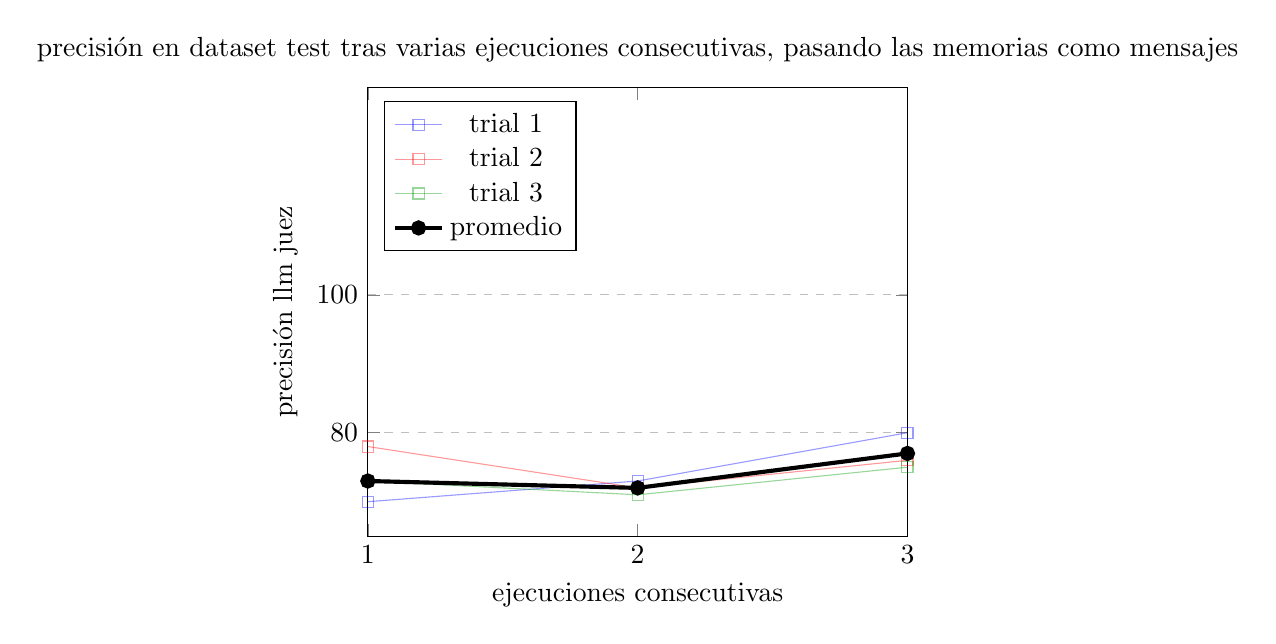
\begin{tikzpicture}
\begin{axis}[
    title={precisión en dataset test tras varias ejecuciones consecutivas, pasando las memorias como mensajes},
    xlabel={ejecuciones consecutivas},
    ylabel={precisión llm juez},
    xmin=1, xmax=3,
    ymin=65, ymax=130,
    xtick={1, 2, 3},
    ytick={0,20,40,60,80,100},
    legend pos=north west,
    ymajorgrids=true,
    grid style=dashed,
]
% gráfico original de solubilidad
\addplot[
    color=blue,
    mark=square,
    opacity=0.4,
    ]
    coordinates {
    (1, 70)(2, 73)(3, 80) 
    };
% primer punto adicional 
\addplot[
    color=red,
    mark=square,
    opacity=0.4,
    ]
    coordinates {
      (1, 78)(2, 72)(3, 76)
    };
% segundo punto adicional 
\addplot[
    color=green!60!black,
    mark=square,
    opacity=0.4,
    ]
    coordinates {
      (1, 73)(2, 71)(3, 75)
    };
% línea promedio
\addplot[
    color=black,
    mark=*,
    line width=1.5pt,
    ]
    coordinates {
      (1, 73)(2, 72)(3, 77)
    };
\legend{trial 1, trial 2, trial 3, promedio}
    
\end{axis}
\end{tikzpicture}

media sin memorias: 76
con memorias train: 81, 83,78 
media con memorias train: 80.66

